%%%%%%%%%%%%%%%%%%%%%%%%%%%%%%%%%%%%%%%%%%%%%%%%%%%%%%%%%%%%%%%%%%%%%%%%%%%%%%
%%
%% This file is part of the ASTERICS Framework. 
%%
%% Copyright (C) Hochschule Augsburg, University of Applied Sciences
%% Efficient Embedded Systems Group
%%
%% Author(s): Philip Manke <philip.manke@hs-augsburg.de>
%%
%%%%%%%%%%%%%%%%%%%%%%%%%%%%%%%%%%%%%%%%%%%%%%%%%%%%%%%%%%%%%%%%%%%%%%%%%%%%%%





%%%%%%%%%%%%%%%%%%%%%%%%%%%%% 7.5. i2c Master %%%%%%%%%%%%%%%%%%%%%%%%%%%%%%%%


\subsection{\textit{i2c} Bus Master} 
\label{ch:07-05-modules-i2c}
\secauthor{Philip Manke}

This section describes the module \texttt{as\_iic} in detail.
\texttt{as\_iic} implements a simple \textit{i2c} master with relatively limited functionality.


\subsubsection{General Overview of Features and Limitations}

The entire module was developed with a mindset of keeping the hardware small and adding only the most important features. Its primary use-case is configuring the cameras that are used with \asterics.

Figure \ref{07-05-as-iic-overview} gives a general overview of the ports of the module. 

\begin{figure}[htbp]
\noindent \begin{centering}
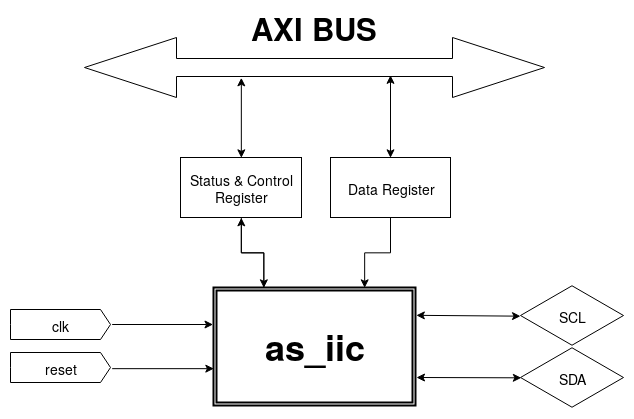
\includegraphics[width=\textwidth]{figs/07-05-as-iic-module-overview}
\par\end{centering}
\caption{Interfaces of the \texttt{as\_iic} hardware module}
\label{07-05-as-iic-overview}
\end{figure}

The following features are supported:

\begin{itemize}
	\item \textit{standard} and \textit{fast mode} \textit{i2c}.
	\item Variable bus clock (configurable via software) of frequencies between 10 kHz to 1 MHz
	\item Clock stretching
	\item 7 bit addressing
	\item Multi-byte transactions
	\item Master-acknowledge
\end{itemize}

\bigskip

The modules limitations are:

\begin{itemize}
	\item Only 8 bit addressing.
	\item No arbitration of any kind. Therefore, multi-master configurations are not supported.
	\item No faster modes of operation than Fast Mode.
	\item No interrupt support. The driver utilizes polling.
	\item No buffering of data. The driver has to transfer each byte sequentially.
\end{itemize}

10 bit addressing is possible with the current hardware, though it hasn't been implemented by the driver.

\subsubsection{The Hardware}

The hardware core consists of two state machines: one handles the generation of the bus clock (SCL) and the other controls the data signal (SDA) and the behaviour of the entire module.

\subsubsection*{The interfaces of \texttt{as\_iic}}

The \texttt{as\_iic} module requires two 32 bit slave registers on an AXI-Slave bus.
The first register is a combined status and control register, which also transfers the data received from the \textit{i2c} slave. 
The second register is read-only for the \texttt{as\_iic} hardware and is used to transfer the data to send to the \textit{i2c} bus and for configuring the \textit{i2c} bus clock frequency.

The status and control register is provided as three 16 bit registers for the status bits, the control bits and a special control-reset register respectively.
The control-reset register allows the AXI-Bus to reset control bits by itself.
If a bit in the control-reset register goes high, the respective bit in the control register is automatically set to low.
Table \ref{07-05-as-iic-registers} gives an overview of the registers of \texttt{as\_iic}.

\begin{longtable}[htb]{|c|c|c|c|}
\hline 
\textbf{Register Name} & \textbf{Access} & \textbf{Offset} & \textbf{Description} \\
\hline
\endhead

\texttt{Status \& Control Register} & RW & 1 &
\parbox{7cm}{ ~ \\ Status and control register for the hardware \\ ~ \\ \small
Half of this register reports the current status of the hardware module of \texttt{as\_iis} to the software. It is also used to transfer bytes, received from slaves on the \textit{i2c} bus, to the software.
The other half is used to control the hardware.
\\ ~ } \\

\hline 

\texttt{Data Register} & W & 0 &
\parbox{7cm}{ ~ \\ Data register for the hardware \\ ~ \\ \small
This register is used to control the hardware module.
Transactions can be initiated, stopped and modified, using bits of this register.
It also contains a soft reset bit.
\\ ~ } \\

\hline 

\caption{The registers of \texttt{as\_iic}}
\label{07-05-as-iic-registers}
\end{longtable}


The tables \ref{07-05-as-iic-control-bits} and \ref{07-05-as-iic-status-bits} explain the purpose of each control and status bit in more detail.

\begin{longtable}[htb]{|c|c|c|c|}
\hline 
\textbf{Bit Name} & \textbf{Access} & \textbf{Index} & \textbf{Description} \\
\hline
\endhead

\texttt{Start/Continue} & W & 0 &
\parbox{9cm}{ ~ \\ Start or continue a transaction. \\ ~ \small
This control bit is used to initiate a transaction from the ready state or continue a transaction for another byte after sending or checking for an acknowledge.
This bit is reset after sending/receiving a byte to/from the \textit{i2c} bus.
\vspace{0.3em} } \\

\hline 

\texttt{Stop} & W & 1 &
\parbox{9cm}{ ~ \\ Stop a transaction. \\ ~ \small
This control bit overwrites the Start/Continue bit and explicitly stops the current transaction after the next acknowledge or after the start bit.
This bit is reset when the hardware is in the ready state.
\vspace{0.3em} } \\

\hline 

\texttt{Read/Write} & W & 2 &
\parbox{9cm}{ ~ \\ Choose to write or read the next byte. \\ ~ \small
This bit toggles between writing a data byte onto the bus or reading a data byte from the bus.
It is sampled after checking for or sending an acknowledge.
This bit is only reset after stopping a transaction.
The default value is '0' (\^= write).
\vspace{0.3em} } \\

\hline

\texttt{Reset} & W & 3 &
\parbox{9cm}{ ~ \\ Completely reset the hardware. \\ ~ \small
This bit acts just like a hard reset for the \texttt{as\_iic} module.
The hardware will enter the ready state again after just a few clock cycles.
This bit is reset immediately.
\vspace{0.3em} } \\

\hline

\texttt{Data Ready} & W & 4 &
\parbox{9cm}{ ~ \\ Signal the hardware to continue. \\ ~ \small
This bit operates in conjunction with the status bit "Waiting SW".
When that status bit is set, the hardware is waiting for the software to finish setting up the data register for the next data byte or finish reading from the status register.
When the software is done, it needs to set this control bit.
The hardware will then continue with the transaction.
This bit is reset immediately.
\vspace{0.3em} } \\

\hline

\texttt{Ack Mod} & W & 5 &
\parbox{9cm}{ ~ \\ Send a master acknowledge. \\ ~ \small
This bit's only purpose is to tell the hardware to send an acknowledge after sending the \textit{i2c} slave address.
It is reset after sending/receiving a data byte.
\vspace{0.3em} } \\

\hline

\caption{Bit fields of the control register}
\label{07-05-as-iic-control-bits}
\end{longtable}

\begin{longtable}[htb]{|c|c|c|c|}
\hline 
\textbf{Bit Name} & \textbf{Access} & \textbf{Bit} & \textbf{Description} \\
\hline
\endhead


\texttt{IIC Ready} & R & 0 &
\parbox{8,5cm}{ ~ \\ The module's hardware is ready. \\ ~ \\ \small
This status bit is only set when the hardware is in the ready state.
\\ ~ } \\

\hline

\texttt{IO Ready} & R & 1 &
\parbox{8,5cm}{ ~ \\ The AXI Slave Registers are safe to read/write. \\ ~ \\ \small
When this status bit is set, the hardware is currently not reading/writing from/to the data byte parts of the AXI Slave registers, meaning that IO operations are allowed and safe.
\\ ~ } \\

\hline

\texttt{Bus Active} & R & 2 &
\parbox{8,5cm}{ ~ \\ This module is active on the \textit{i2c} bus. \\ ~ \\ \small
This status bit is always set when the \texttt{as\_iic} module is actively setting the SDA signal of the \textit{i2c} bus.
\\ ~ } \\

\hline

\texttt{Ack Rec} & R & 3 &
\parbox{8,5cm}{ ~ \\ Acknowledgement was received. \\ ~ \\ \small
This bit is set after checking for an acknowledgement bit from the slave after sending a data byte to the \textit{i2c} bus.
It should only be sampled after a write transaction as the value is only valid then.
Also note that this bit can only report on the state of the acknowledgement from the previous data byte.
It is reset just before checking for an acknowledge bit or when starting a new transaction.
\\ ~ } \\

\hline

\texttt{Stalled} & R & 4 &
\parbox{8,5cm}{ ~ \\ Clock stretching is detected. \\ ~ \\ \small
This bit is set every time clock stretching is detected.
Note that it is accurate to within a single system clock cycle.
The bit is reset immediately after the slave releases SCL.
\\ ~ } \\

\hline

\texttt{Waiting SW} & R & 5 &
\parbox{8,5cm}{ ~ \\ The hardware is waiting for the software. \\ ~ \\ \small
This bit is working in conjunction with the control bit "Data Ready".
When this bit is set, the hardware is waiting on the control bit "Data Ready" to be set by the software.
The hardware will always wait after sending/receiving a byte, before sending/checking for an acknowledge.
This allows the software to finish tasks like reading the last received data byte and writing the next data byte to be send.
This bit is immediately reset after the software sets "Data Ready".
\\ ~ } \\

\hline

\textit{Unused} & R & 6 - 7 &
\parbox{8,5cm}{ ~ \\ Unused \\ ~ \\ \small
\\ ~ } \\

\hline

\texttt{Data RX} & R & 8 - 15 &
\parbox{8,5cm}{ ~ \\ Data received from the bus \\ ~ \\ \small
This part of the status register is used by the hardware to transfer data received from slave devices on the bus to the software.
\\ ~ } \\

\hline


\caption{Bit fields of the status register}
\label{07-05-as-iic-status-bits}
\end{longtable}

\begin{longtable}[htb]{|c|c|c|c|}
\hline 
\textbf{Bit Name} & \textbf{Access} & \textbf{Bit} & \textbf{Description} \\
\hline
\endhead

\texttt{SCL\_DIV} & W & 0 - 23 &
\parbox{8,5cm}{ ~ \\ SCL counter compare value \\ ~ \\ \small
This value is used to reset the SCL counter, which is used to generate the \textit{i2c} bus frequency.
\\ ~ } \\

\hline 

\texttt{Data TX} & W & 24 - 31 &
\parbox{8,5cm}{ ~ \\ Data to send to the \textit{i2c} bus \\ ~ \\ \small
This part of the data register is used to transfer the bytes for the hardware to send on the bus.
\\ ~ } \\

\hline 

\caption{Bit fields of the data register}
\label{07-05-as-iic-data-register}
\end{longtable}

Besides the registers, there are the clock and hardware reset signals that go into the module and the SCL and SDA signals for the \textit{i2c} bus, which are "inout" signals, driven by the module using tristate drivers.
These signals should be connected to the outside using GPIO Pins connected to the \textit{i2c} devices, you wish to communicate with.
Though not intended, an internal \textit{i2c} bus could be configured just the same.

\subsubsection*{Generation of the SCL signal}

The data width used to configure the frequency for SCL differs, depending on the hardware configuration. It is always equal to the value of the "SCL\_DIV\_REGISTER\_WIDTH" generic, configurable before synthesis.
The data is little endian.

"SCL\_DIV\_REGISTER\_WIDTH", the modules only generic, sets the size of the counter that is used to detect when to switch the SCL signal. Therefore a wider counter allows for lower frequencies on the bus.
Also: With higher system clock frequencies a wider SCL DIV counter might be necessary to achieve the desired \textit{i2c} bus clock frequency.

The value used to configure the counter compare value in the data register (SCL\_DIV), is calculated as follows:

\[RegisterValue = (SystemFrequency / (4 * DesiredBusFrequency)) - 2 \]

With that, the ideal value for the "SCL\_DIV\_REGISTER\_WIDTH" generic is:

\[\log_{2}(RegisterValue)\]

Where the \textit{SystemFrequency} is the frequency of the clock driving the \texttt{as\_iic} module, \textit{DesiredBusFrequency} is the desired frequency of the SCL signal on the \textit{i2c} bus and \textit{RegisterValue} is the value to set the "Frequency for SCL" part of the data register to.\\
Note that the practical minimum value for the register value is 3.
This will run the hardware as fast as possible.

A state machine in conjunction with the aforementioned counter is used to generate the SCL clock signal. Every time the counter reaches the compare value configured via the data register, it is reset and a separate modulo 4 counter is incremented. Bit 1 of this smaller counter corresponds to the state of the SCL signal.
This also means that every time bit 0 of this smaller counter changes, one quarter of the bus clock period has passed.
This is an important signal for many parts of the hardware, as it changes exactly between and on the edges of the SCL clock signal.
Figure \ref{07-05-as-iic-scl-generation} shows a simplified diagram of the counters involved in generating the SCL signal.

\begin{figure}[htbp]
\noindent \begin{centering}
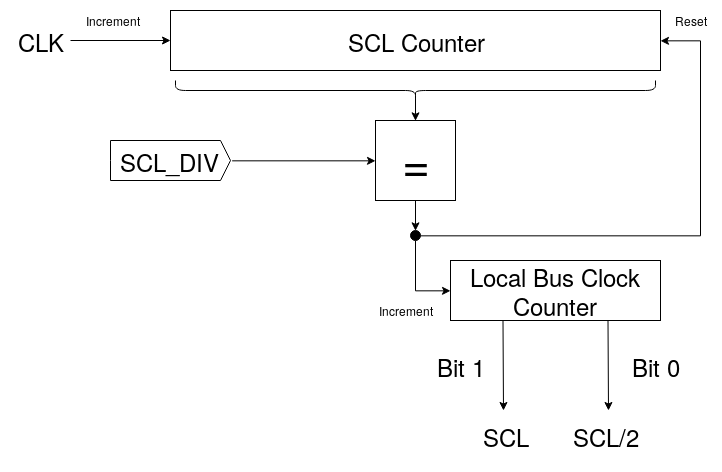
\includegraphics[width=\textwidth]{figs/07-05-as-iic-scl-generation}
\par\end{centering}
\caption{The counters generating the SCL Signal in \texttt{as\_iic}}
\label{07-05-as-iic-scl-generation}
\end{figure}

The state machine controls the counters and sets the SCL signal according to the mod 4 counter's state.
The "mod 4 counter" is also called \textit{local bus clock} or \textit{local bus clock counter} in hardware and in the graphic.
It also sets the "stalled" status signal, whenever clock stretching is detected.
This is done by monitoring the SCL bus signal and comparing it to the internal SCL signal (\textit{lbclk}).
If the signals differ from each other, another device on the \textit{i2c} bus is interfering with the clock signal (\^= "clock stretching").


\subsubsection*{The SDA state machine}

\begin{figure}[htbp]
\noindent \begin{centering}
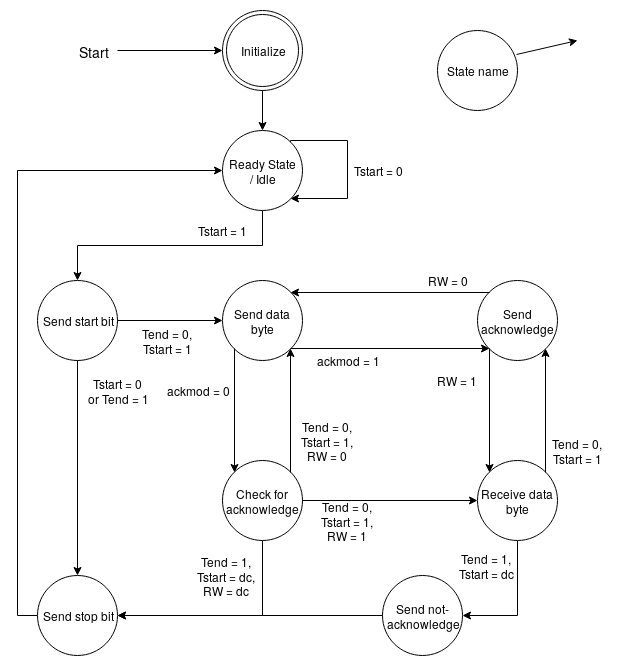
\includegraphics[width=\textwidth]{figs/07-05-as-iic-statemachine}
\par\end{centering}
\caption{Visualization of the SDA state machine in \texttt{as\_iic}}
\label{07-05-as-iic-states}
\end{figure}

This second larger state machine is used to control the SDA signal, manage the communication with the software via the AXI-Bus and manage the SCL state machine.\\
The states of this state machine can be grouped to correspond to different sections of the \textit{i2c} protocol, as seen in figure \ref{07-05-as-iic-states}.

The state machine oftentimes uses the \textit{i2c} bus signals SDA and SCL as parameters.
When it does that, these signals are not the internal signals, but are read directly from the bus, to make sure that clock stretching is always recognized.\\
When setting or sampling the SDA signal while sending or receiving a data byte, bit 0 from the \textit{local bus clock counter} (\textit{lbclk\_half}) is used as the trigger.
When this bit of the counter changes, exactly one quarter of the SCL clock period has passed, meaning that this is exactly in between two SCL clock edges. This guards against possible timing violations.

\subsubsection*{The "Master Acknowledge"}

A non-standard feature supported by this \textit{i2c} master implementation is the \textit{Master-Acknowledge}. After the slave address has been sent to the bus, the master is able to send an acknowledge bit by itself.
This behaviour is controlled by the software through the \texttt{ack\_mod} control bit. 
Some driver functions, like \texttt{set\_regpointer}, use this functionality and some functions take an additional parameter, the \texttt{modifier} byte, which can enable this and other functionality.

\subsubsection*{How to connect a hardware module to the \textit{i2c} bus} \label{07-05-as-iic-connect-devices}

As mentioned before the \textit{i2c} bus consists of just two signals/wires: SCL and SDA.
To connect a new slave device to the bus, these two wires of the \texttt{as\_iic} master need to be connected to the appropriate wires of the slave.
The SCL wires are connected together and the SDA wires are connected together.\\
The \textit{i2c} bus requires that each signal has a pull-up resistor connected to it.
This requires a resistor of between 1 kilo ohm and 10 kilo ohm to be connected to the signal and the supply voltage (usually 3.3 Volts) for both signals.

Possible problems with the \textit{i2c} bus include:

\begin{itemize}
	\item Multiple pull-up resistors present per signal
	\item Capacitance between the signals and ground is too high
	\item Interference from other signals
\end{itemize}

For more in-depth knowledge on the design of the hardware, consider looking through the VHDL source files of \texttt{as\_iic} available in \texttt{"modules/as\_iic/hardware/"}.

\subsubsection*{Waveform examples}

This section will further explain the \textit{i2c} protocol, using some waveform examples.\\
Figure \ref{07-05-as-iic-wave-write} shows some signals of a simulated \texttt{as\_iic} during a write operation.

\begin{figure}[htbp]
\noindent \begin{centering}
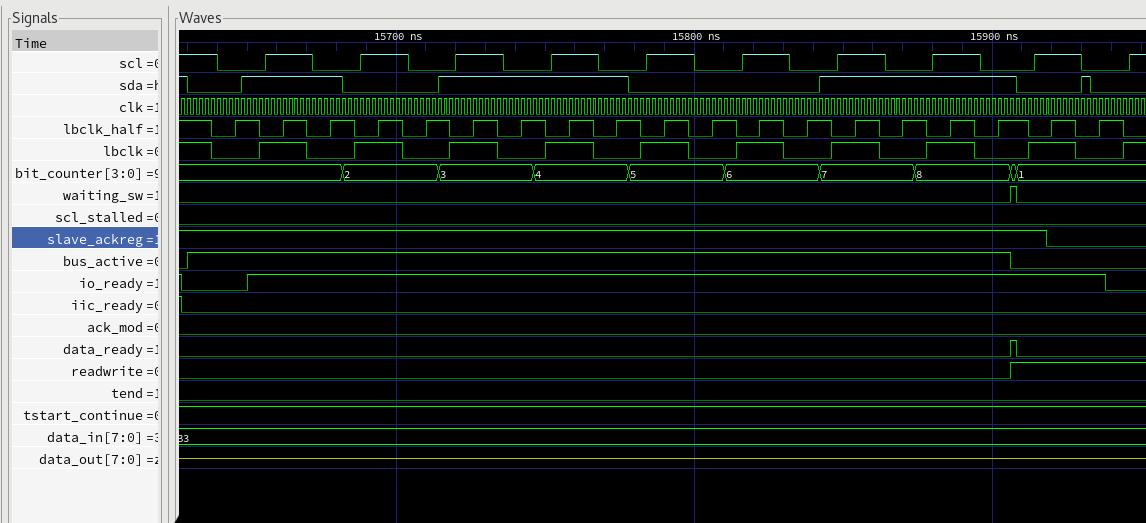
\includegraphics[width=\textwidth]{figs/07-05-as-iic-wave-write}
\par\end{centering}
\caption{\textit{i2c} read transaction as a waveform from a simulated \texttt{as\_iic} module}
\label{07-05-as-iic-wave-write}
\end{figure}

The first operation shown is the start bit, SDA going low while SCL is high followed by SCL going low while SDA is still low.
Following that, SDA may change while SCL is low and has to be valid when SCL goes high.\\
Furthermore some \texttt{as\_iic} specific relations can be demonstrated using this waveform.
The relationship between the system clock \texttt{clk}, the local bus clock counter, \texttt{lbclk} (\^= bit 1) and \texttt{lbclk\_half} (\^= bit 0), SCL and SDA where SCL is equal to \texttt{lbclk} but slightly delayed and SDA changes slightly after \texttt{lbclk\_half} goes high.

Figure \ref{07-05-as-iic-wave-read} shows a read transaction from the same simulated module.

\begin{figure}[htbp]
\noindent \begin{centering}
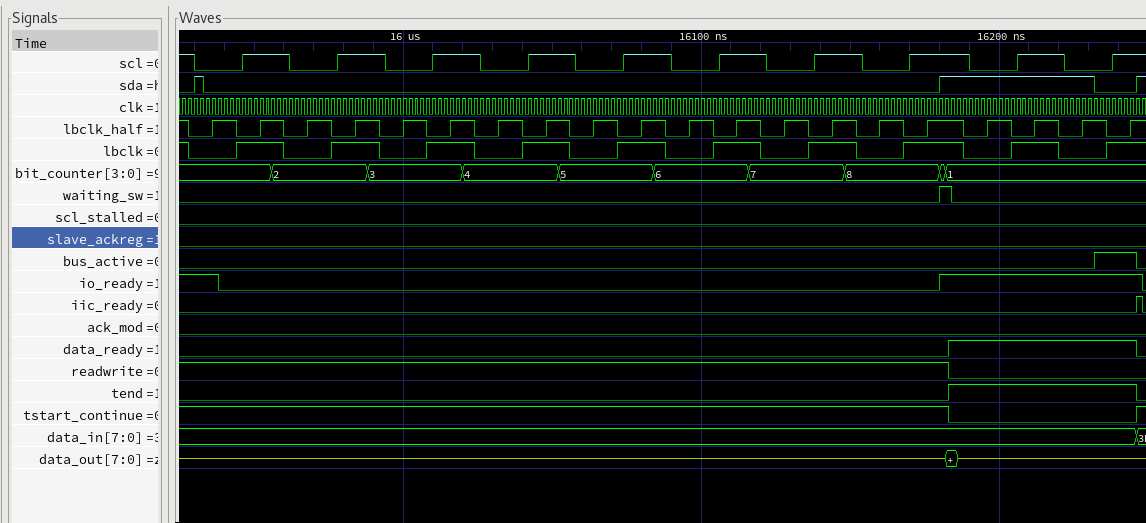
\includegraphics[width=\textwidth]{figs/07-05-as-iic-wave-read}
\par\end{centering}
\caption{\textit{i2c} write transaction as a waveform from a simulated \texttt{as\_iic} module}
\label{07-05-as-iic-wave-read}
\end{figure}

Finally figure \ref{07-05-as-iic-wave-real} shows a complete read transaction and write transaction captured using a logic analyzer using real hardware.
In this figure the start bits are marked by a green circle and the stop bits by a red circle.
Every transferred bit is marked by a small arrow on the edge of SCL going high, with the clock cycle for the acknowledge lacking this arrow.

\begin{figure}[htbp]
\noindent \begin{centering}
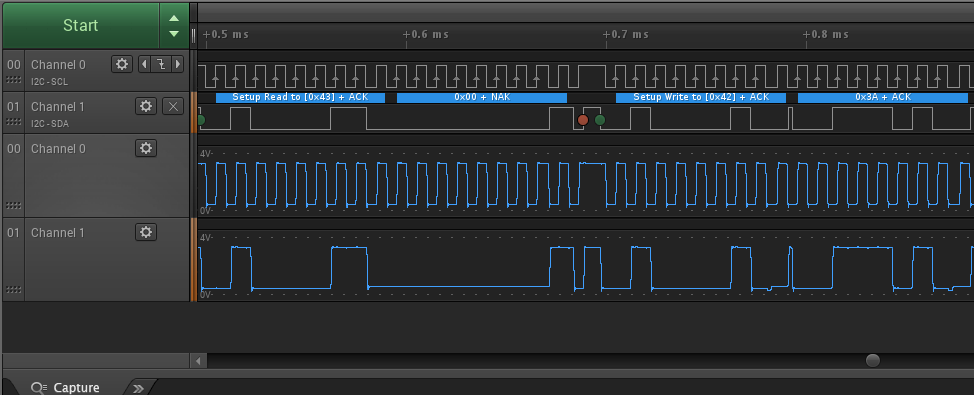
\includegraphics[width=\textwidth]{figs/07-05-as-iic-wave-real}
\par\end{centering}
\caption{Waveform captured using a logic analyzer from the \texttt{as\_iic} module}
\label{07-05-as-iic-wave-real}
\end{figure}

\subsubsection{The Software Driver}

The driver's low level functions are built to act as a modular system.
A few low level functions can be put together to a sequence, which can act as any possible \textit{i2c} transaction the hardware supports.
This means that less knowledge of this particular hard- and software implementation is required to expand the drivers functionality.
All of the lower level functions reference "transactions". This refers to all the actions between and including the start bit and the stop bit, meaning a transaction can contain an arbitrary count of data bytes.

The higher level functions can be used as is, after initializing the module properly.
They include single byte transactions, multi-byte transactions and transactions which refer to "registers" or "reg(s)".
This refers to registers of the \textit{i2c} slaves on the bus.

Table \ref{07-05-as-iic-functions} provides an overview of the transactions available in the driver.

\begin{table}[htb]
	\centering
	\begin{tabular}[t]{|r|l|}
		\hline
		\textbf{Function Name} & \textbf{Transaction Type}\\ \hline
		as\_iic\_write\_byte & Single Byte Write\\ \hline
		as\_iic\_get\_byte & Single Byte Read\\ \hline
		as\_iic\_write\_bytes & Multi-Byte Write\\ \hline
		as\_iic\_read\_bytes & Multi-Byte Read\\ \hline
		as\_iic\_write\_reg & Set an \textit{i2c} Device's Slave Register\\ \hline
		as\_iic\_read\_reg & Read an \textit{i2c} Device's Slave Register\\ \hline
		as\_iic\_read\_regs & Read successive Slave Registers\\ \hline
		as\_iic\_set\_regpointer & Set special Slave Register (Master ACK)\\ \hline
	\end{tabular}
	
	\caption{Listing of the high-level functions available for \texttt{as\_iic}}
	\label{07-05-as-iic-functions}
\end{table}

For more information on the high level functions and the lower level functions not mentioned here, see the \asterics Doxygen driver documentation.


\subsubsection{Quirks of \texttt{as\_iic}} \label{07-05-04-as-iic-quirks}

\subsubsection*{Hard Wait Mechanism}

The driver has a hard-coded wait mechanism that waits for about 50 us after every transaction to give the slave enough time to recognize the end and start of two sequential transactions.  

\subsubsection*{SCL Frequency Configuration}

The configuration for the SCL frequency is immediately applied in the hardware. 
The valid frequencies range from 10kHz to 1MHz. Note though, that the entire range is not always supported by the specific hardware configuration.
This means, that the frequency can be set to a value that the \texttt{as\_iic} hardware can not handle.
The minimum value for the SCL configuration register is 3.
The maximum is dependent on your hardware configuration of \asterics.
Note that the frequency configuration is NOT reset when calling the reset-function \texttt{as\_iic\_reset\_hw\_state()} and is only reset by the function \texttt{as\_iic\_reset()}.

\subsubsection*{Pull-up Resistors for the \textit{i2c} Bus}

The \texttt{as\_iic} module does not configure internal pull-up resistors for the \textit{i2c} signals, as the internally provided current is usually too weak. Therefore external pull-up resistors have to be provided by the user in order to use the \texttt{as\_iic} module.
The section \ref{07-05-as-iic-connect-devices} briefly covers how to connect devices to the \textit{i2c} bus and how to connect the required pull-up resistors.

